% -*- TeX-engine: xetex; eval: (auto-fill-mode 0); eval: (visual-line-mode 1); -*-
% Compile with XeLaTeX

%%%%%%%%%%%%%%%%%%%%%%%
% Option 1: Slides: (comment for handouts)   %
%%%%%%%%%%%%%%%%%%%%%%%

%\documentclass[slidestop,compress,mathserif,12pt,t,professionalfonts,xcolor=table]{beamer}
%
%% solution stuff
%\newcommand{\solnMult}[1]{
%\only<1>{#1}
%\only<2->{\red{\textbf{#1}}}
%}
%\newcommand{\soln}[1]{\textit{#1}}

%%%%%%%%%%%%%%%%%%%%%%%%%%%%%%%
% Option 2: Handouts, without solutions (post before class)    %
%%%%%%%%%%%%%%%%%%%%%%%%%%%%%%%

 \documentclass[11pt,containsverbatim,handout,xcolor=xelatex,dvipsnames,table]{beamer}

 % handout layout
 \usepackage{pgfpages}
 \pgfpagesuselayout{4 on 1}[letterpaper,landscape,border shrink=5mm]

 % solution stuff
 \newcommand{\solnMult}[1]{#1}
 \newcommand{\soln}[1]{}

%%%%%%%%%%%%%%%%%%%%%%%%%%%%%%%%%%%%
% Option 3: Handouts, with solutions (may post after class if need be)    %
%%%%%%%%%%%%%%%%%%%%%%%%%%%%%%%%%%%%

% \documentclass[11pt,containsverbatim,handout,xcolor=xelatex,dvipsnames,table]{beamer}

% % handout layout
% \usepackage{pgfpages}
% \pgfpagesuselayout{4 on 1}[letterpaper,landscape,border shrink=5mm]

% % solution stuff
% \newcommand{\solnMult}[1]{\red{\textbf{#1}}}
% \newcommand{\soln}[1]{\textit{#1}}

%%%%%%%%%%
% Load style file, defaults  %
%%%%%%%%%%

%%%%%%%%%%%%%%%%
% Themes
%%%%%%%%%%%%%%%%

% See http://deic.uab.es/~iblanes/beamer_gallery/ for mor options

% Style theme
\usetheme{metropolis}

% Color theme
%\usecolortheme{seahorse}

% Helvetica Neue Light for most text
%\usepackage{fontspec}
%\setsansfont{Helvetica Neue Light}

%%%%%%%%%%%%%%%%
% Packages
%%%%%%%%%%%%%%%%

\usepackage{geometry}
\usepackage{graphicx}
\usepackage{amssymb}
\usepackage{epstopdf}
\usepackage{amsmath}  	% this permits text in eqnarray among other benefits
\usepackage{url}		% produces hyperlinks
\usepackage[english]{babel}
\usepackage{colortbl}	% allows for color usage in tables
\usepackage{multirow}	% allows for rows that span multiple rows in tables
\usepackage{color}		% this package has a variety of color options
\usepackage{pgf}
\usepackage{calc}
\usepackage{ulem}
\usepackage{multicol}
\usepackage{textcomp}
\usepackage{listings}
\usepackage{changepage}
\usepackage{tikz}
\usetikzlibrary{trees}		% for probability trees
\usepackage{fancyvrb}	% for colored code chunks
\usepackage{nameref}

%%%%%%%%%%%%%%%%
% Remove navigation symbols
%%%%%%%%%%%%%%%%

\beamertemplatenavigationsymbolsempty
\hypersetup{pdfpagemode=UseNone} % don't show bookmarks on initial view

%%%%%%%%%%%%%%%%
% User defined colors
%%%%%%%%%%%%%%%%

% Pantone 2016 Spring colors
% https://atelierbram.github.io/c-tiles16/colorscheming/pantone-spring-2016-colortable.html
% update each semester or year

\xdefinecolor{custom_blue}{rgb}{0.01, 0.31, 0.52} % Snorkel Blue
\xdefinecolor{custom_darkBlue}{rgb}{0.20, 0.20, 0.39} % Reflecting Pond  
\xdefinecolor{custom_orange}{rgb}{0.96, 0.57, 0.42} % Cadmium Orange
\xdefinecolor{custom_green}{rgb}{0, 0.47, 0.52} % Biscay Bay
\xdefinecolor{custom_red}{rgb}{0.58, 0.32, 0.32} % Marsala

\xdefinecolor{custom_lightGray}{rgb}{0.78, 0.80, 0.80} % Glacier Gray
\xdefinecolor{custom_darkGray}{rgb}{0.35, 0.39, 0.43} % Stormy Weather

%%%%%%%%%%%%%%%%
% Template colors
%%%%%%%%%%%%%%%%

%\setbeamercolor*{palette primary}{fg=white,bg= custom_blue}
%\setbeamercolor*{palette secondary}{fg=black,bg= custom_blue!80!black}
%\setbeamercolor*{palette tertiary}{fg=white,bg= custom_blue!80!black!80}
%\setbeamercolor*{palette quaternary}{fg=white,bg= custom_blue}
%
%\setbeamercolor{structure}{fg= custom_blue}
%\setbeamercolor{frametitle}{bg= custom_blue!90}
%\setbeamertemplate{blocks}[shadow=false]
%\setbeamersize{text margin left=2em,text margin right=2em}

%%%%%%%%%%%%%%%%
% Styling fonts, bullets, etc.
%%%%%%%%%%%%%%%%
%
%% title slide
%\setbeamerfont{title}{size=\large,series=\bfseries}
%\setbeamerfont{subtitle}{size=\large,series=\mdseries}
%%\setbeamerfont{institute}{size=\large,series=\mdseries}
%
% color of alerted text
\setbeamercolor{alerted text}{fg=custom_orange}

% styling of itemize bullets
\setbeamercolor{item}{fg=custom_blue}
\setbeamertemplate{itemize item}{{{\small$\blacktriangleright$}}}
\setbeamercolor{subitem}{fg=custom_blue}
\setbeamertemplate{itemize subitem}{{\textendash}}
\setbeamerfont{itemize/enumerate subbody}{size=\footnotesize}
\setbeamerfont{itemize/enumerate subitem}{size=\footnotesize}

% styling of enumerate bullets
\setbeamertemplate{enumerate item}{\insertenumlabel.}

%\setbeamerfont{enumerate item}{family={\fontspec{Helvetica Neue}}}
%\setbeamerfont{enumerate subitem}{family={\fontspec{Helvetica Neue}}}
%\setbeamerfont{enumerate subsubitem}{family={\fontspec{Helvetica Neue}}}

% make frame titles small to make room in the slide
\setbeamerfont{frametitle}{size=\small} 




%% set Helvetica Neue font for frame and section titles
%\setbeamerfont{frametitle}{family={\fontspec{Helvetica Neue}}}
%\setbeamerfont{sectiontitle}{family={\fontspec{Helvetica Neue}}}
%\setbeamerfont{section in toc}{family={\fontspec{Helvetica Neue}}}
%\setbeamerfont{subsection in toc}{family={\fontspec{Helvetica Neue}}, size=\small}
%\setbeamerfont{footline}{family={\fontspec{Helvetica Neue}}}
%\setbeamerfont{subsection in toc}{family={\fontspec{Helvetica Neue}}}
%\setbeamerfont{block title}{family={\fontspec{Helvetica Neue}}}
%
%%%%%%%%%%%%%%%%%
%% New fonts accessed by fontspec package
%%%%%%%%%%%%%%%%%
%
%% Monaco font for code
%\newfontfamily{\monaco}{Monaco}

%%%%%%%%%%%%%%%%
% Color text commands
%%%%%%%%%%%%%%%%

%orange
\newcommand{\orange}[1]{\textit{\textcolor{custom_orange}{#1}}}

% yellow
\newcommand{\yellow}[1]{\textit{\textcolor{yellow}{#1}}}

% blue
\newcommand{\blue}[1]{\textit{\textcolor{blue}{#1}}}

% green
\newcommand{\green}[1]{\textit{\textcolor{custom_green}{#1}}}

% red
\newcommand{\red}[1]{\textit{\textcolor{custom_red}{#1}}}

% dark gray
\newcommand{\darkgray}[1]{\textit{\textcolor{custom_darkGray}{#1}}}

% light gray
\newcommand{\lightgray}[1]{\textit{\textcolor{custom_lightGray}{#1}}}

% pink
\newcommand{\pink}[1]{\textit{\textcolor{pink}{#1}}}


%%%%%%%%%%%%%%%%
% Custom commands
%%%%%%%%%%%%%%%%

% empty box for probability tree frame
\newcommand{\emptybox}[2]{
	\fbox{ \begin{minipage}{#1} \hfill\vspace{#2} \end{minipage} }
}

% cancel
\newcommand{\cancel}[1]{%
    \tikz[baseline=(tocancel.base)]{
        \node[inner sep=0pt,outer sep=0pt] (tocancel) {#1};
        \draw[red, line width=0.5mm] (tocancel.south west) -- (tocancel.north east);
    }%
}

% degree
\newcommand{\degree}{\ensuremath{^\circ}}

% cite
\newcommand{\ct}[1]{
\vfill
{\tiny #1}}

% Note
\newcommand{\Note}[1]{
\rule{2.5cm}{0.25pt} \\ \textit{\footnotesize{\textcolor{custom_red}{Note:} \textcolor{custom_darkGray}{#1}}}}

% Remember
\newcommand{\Remember}[1]{\textit{\scriptsize{\textcolor{custom_red}{Remember:} #1}}}

% links: webURL, webLink
\newcommand{\webURL}[1]{\urlstyle{same}{\textit{\textcolor{custom_blue}{\url{#1}}}}}
\newcommand{\webLink}[2]{\href{#1}{\textcolor{custom_blue}{{#2}}}}

% mail
\newcommand{\mail}[1]{\href{mailto:#1}{\textit{\textcolor{custom_blue}{#1}}}}

% highlighting: hl, hlGr, mathhl
\newcommand{\hl}[1]{\textit{\textcolor{custom_blue}{#1}}}
\newcommand{\hlGr}[1]{\textit{\textcolor{custom_green}{#1}}}
\newcommand{\mathhl}[1]{\textcolor{custom_blue}{\ensuremath{#1}}}

% example
\newcommand{\ex}[1]{\textcolor{blue}{{{\small (#1)}}}}

% twocol: two columns
\newenvironment{twocol}[4]{
\begin{columns}[c]
\column{#1\textwidth}
#3
\column{#2\textwidth}
#4
\end{columns}
}

% threecol: three columns
\newenvironment{threecol}[6]{
\begin{columns}[c]
\column{#1\textwidth}
#4
\column{#2\textwidth}
#5
\column{#3\textwidth}
#6
\end{columns}
}

% slot (for probability calculations)
\newenvironment{slot}[2]{
\begin{array}{c} 
\underline{#1} \\ 
#2
\end{array}
}

% pr: left and right parentheses
\newcommand{\pr}[1]{
\left( #1 \right)
}

%%%%%%%%%%%%%%%%
% Custom blocks
%%%%%%%%%%%%%%%%

% activity: less commonly used
\newcommand{\activity}[2]{
\setbeamertemplate{itemize item}{{{\small\textcolor{custom_orange}{$\blacktriangleright$}}}}
\setbeamercolor{block title}{fg=white, bg=custom_orange}
\setbeamerfont{block title}{size=\small}
\setbeamercolor{block body}{fg=black, bg=custom_orange!20!white!80}
\setbeamerfont{block body}{size=\small}
\begin{block}{Activity: #1}
\setlength\abovedisplayskip{0pt}
#2
\end{block}
}

% app: application exercise
\newcommand{\app}[2]{
\setbeamercolor{block title}{fg=white,bg=custom_green}
\setbeamercolor{block body}{fg=black,bg=custom_green!20!white!80}
\begin{block}{{\small Application exercise: #1}}
#2
\end{block}
}

% disc: discussion question
\newcommand{\disc}[1]{
\vspace*{-2ex}
\setbeamercolor{block body}{bg=custom_blue!25!white!80, fg=custom_blue!55!black!95}
\begin{block}{\vspace*{-3ex}}
#1
\end{block}
\vspace*{-1ex}
}

% clicker: clicker question
\newcommand{\clicker}[1]{
\setbeamercolor{block title}{bg=custom_blue!80!white!50,fg=custom_blue!30!black!90}
\setbeamercolor{block body}{bg=custom_blue!20!white!80,fg=custom_blue!30!black!90}
\begin{block}{\vspace*{-0.2ex}{\footnotesize Your turn}\vspace*{-0.2ex}}
#1
\end{block}
}

% formula
\newcommand{\formula}[2]{
\setbeamercolor{block title}{bg=custom_blue!40!white!60,fg=custom_blue!55!black!95}
\begin{block}{{\small#1}}
#2
\end{block}
}

% code
\newcommand{\Rcode}[1]{
{\monaco {\footnotesize \textcolor{custom_darkBlue}{#1}}}
}

% output
\newcommand{\Rout}[1]{
{\monaco {\footnotesize \textcolor{custom_darkGray}{#1}}}
}

%%%%%%%%%%%%%%%%
% Change margin
%%%%%%%%%%%%%%%%

\newenvironment{changemargin}[2]{%
\begin{list}{}{%
\setlength{\topsep}{0pt}%
\setlength{\leftmargin}{#1}%
\setlength{\rightmargin}{#2}%
\setlength{\listparindent}{\parindent}%
\setlength{\itemindent}{\parindent}%
\setlength{\parsep}{\parskip}%
}%
\item}{\end{list}}

%%%%%%%%%%%%%%%%
% Footnote
%%%%%%%%%%%%%%%%

\long\def\symbolfootnote[#1]#2{\begingroup%
\def\thefootnote{\fnsymbol{footnote}}\footnote[#1]{#2}\endgroup}

%%%%%%%%%%%%%%%%
% Graphics
%%%%%%%%%%%%%%%%

\DeclareGraphicsRule{.tif}{png}{.png}{`convert #1 `dirname #1`/`basename #1 .tif`.png}

%%%%%%%%%%%%%%%%
% Slide number
%%%%%%%%%%%%%%%%

\setbeamertemplate{footline}{%
    \raisebox{5pt}{\makebox[\paperwidth]{\hfill\makebox[20pt]{\color{gray}
          \scriptsize\insertframenumber}}}\hspace*{5pt}}

          
%%%%%%%%%%%%%%%%
% Remove page numbers
%%%%%%%%%%%%%%%%

\newcommand{\removepagenumbers}{% 
  \setbeamertemplate{footline}{}
}

%%%%%%%%%%%%%%%%
% TOC slides
%%%%%%%%%%%%%%%%

\setbeamertemplate{section in toc}{\inserttocsectionnumber.~\inserttocsection}
\setbeamertemplate{subsection in toc}{$\qquad$\inserttocsubsectionnumber.~\inserttocsubsection \\}

\AtBeginSection[] 
{ 
  \addtocounter{framenumber}{-1} 
  % 
  {\removepagenumbers 
  {\small
    \begin{frame}<beamer> 
    \frametitle{Outline} 
    \tableofcontents[currentsection] 
  \end{frame} 
  } 
  }
} 

\AtBeginSubsection[] 
{ 
  \addtocounter{framenumber}{-1} 
  % 
  {\removepagenumbers 
  {\small
    \begin{frame}<beamer> 
    \frametitle{Outline} 
    \tableofcontents[currentsection,currentsubsection] 
  \end{frame} 
  } 
  }
}
% Course Name
\newcommand{\CourseName}{GOVT 3990 - Spring 2017}
\newcommand{\InstituteName}{Cornell University}

% Personal Info
\newcommand{\FirstName}{Sergio}
\newcommand{\LastName}{Garcia-Rios}

% Electronic Info
\newcommand{\PersonalSite}{https://garciarios.github.io}
\newcommand{\CourseSite}{http://garciarios.github.io/govt_3990/}
\newcommand{\Email}{garcia.rios@cornell.edu}

% Exam Dates
\newcommand{\ExamADate}{Feb 24, Wed}
\newcommand{\ExamBDate}{Mar 30, Wed}
\newcommand{\FinalDate}{May 5, Thu - 7-10pm}
% ALT ALT
% % Course Name
\newcommand{\CourseName}{Sta 101 - Spring 2016}
\newcommand{\InstituteName}{Duke University, Department of Statistical Science}

% Personal Info
\newcommand{\FirstName}{Anthea}
\newcommand{\LastName}{Monod}

% Electronic Info
\newcommand{\PersonalSite}{https://stat.duke.edu/people/anthea-monod.html}
\newcommand{\CourseSite}{https://stat.duke.edu/courses/Spring16/sta101.002}
\newcommand{\Email}{anthea@stat.duke.edu}

% Exam Dates
\newcommand{\ExamADate}{Feb 25, Thu}
\newcommand{\ExamBDate}{Mar 31, Thu}
\newcommand{\FinalDate}{???}

%%%%%%%%%%%
% Cover slide info    %
%%%%%%%%%%%

\title{Unit 2: Probability and distributions}
\subtitle{3. Normal and binomial distributions}
\author{\CourseName}
\date{}
\institute{\InstituteName}


%%%%%%%%%%%%%%%%%%%%%%%%%
% Begin document and set Helvetica Neue font   %
%%%%%%%%%%%%%%%%%%%%%%%%%

\begin{document}
\fontspec[Ligatures=TeX]{Helvetica Neue Light}

%%%%%%%%%%%%%%%%%%%%%%%%%%%%%%%%%%%

% Title Page

\begin{frame}[plain]

\titlepage

\vfill

{\scriptsize \webLink{\PersonalSite}{Dr. \LastName{}} \hfill Slides posted at  \webURL{\CourseSite}}

\addtocounter{framenumber}{-1} 

\end{frame}

%%%%%%%%%%%%%%%%%%%%%%%%%%%%%%%%%%%%

\section{Housekeeping}

%%%%%%%%%%%%%%%%%%%%%%%%%%%%%%%%%%%%

\begin{frame}
\frametitle{Announcements}

\begin{itemize}

\item Formatting of problem set submissions:
\begin{itemize}
\item Bad: Scanned PDF handwriting, unreadable/too dark, haphazard orientation of pages, out
of order $\rightarrow$ \red{will result in point deductions if not legible}
\item Better: Scanned PDF \textbf{neat} handwriting, good scan quality, one file containing
all pages in order $\rightarrow$ \red{will result in point deductions if not legible}
\item Best: Typed using a word processor and PDFed
\end{itemize}

\item RA 3 on Wednesday

\item PS 2 due Friday, PA 2 due Sunday

\item Discussion section tomorrow: Normal and binomial distribution problems + any questions regarding Unit 3

\end{itemize}

\end{frame}

%%%%%%%%%%%%%%%%%%%%%%%%%%%%%%%%%%%%

\section{Main ideas}

%%%%%%%%%%%%%%%%%%%%%%%%%%%%%%%%%%%%

\subsection{Two types of probability distributions: discrete and continuous}
\label{mi1}

%%%%%%%%%%%%%%%%%%%%%%%%%%%%%%%%%%%%

\begin{frame}
\frametitle{1. Two types of probability distributions: discrete and continuous}

\begin{itemize}

\item A \hl{discrete probability distribution} lists all possible events and the probabilities with 
which they occur
\begin{itemize}
\item The events listed must be disjoint
\item Each probability must be between 0 and 1 
\item The probabilities must total 1
\end{itemize}
Example: Binomial distribution

\pause

\item A \hl{continuous probability distribution} differs from a discrete probability distribution in 
several ways:
\begin{itemize}
\item The probability that a continuous random variable will equal to any specific value is zero.
\item As such, they cannot be expressed in tabular form.
\item Instead, we use an equation or a formula to describe its distribution via a probability density 
function (pdf).
\item We can calculate the probability for ranges of values the random variable takes (area under 
the curve).
\end{itemize}
Example: Normal distribution

\end{itemize}

\end{frame}

%%%%%%%%%%%%%%%%%%%%%%%%%%%%%%%%%%%%

\subsection{Normal distribution is unimodal, symmetric, and follows the 68-95-99.7 rule}
\label{mi2}

%%%%%%%%%%%%%%%%%%%%%%%%%%%%%%%%%%%%

\begin{frame}
\frametitle{}

\clicker{Speeds of cars on a highway are normally distributed with mean 65 miles / hour. The 
minimum speed recorded is 48 miles / hour and the maximum speed recorded is 83 miles / hour. 
Which of the following is most likely to be the standard deviation of the distribution?}

\begin{enumerate}[(a)]
\item -5 \only<2>{\soln{\darkgray{$\rightarrow$ SD cannot be negative}}}
\item \solnMult{5} \only<2>{\soln{\red{$\rightarrow 65 \pm (3 \times 5) = (50, 80)$}}}
\item 10 \only<2>{\soln{\darkgray{$\rightarrow 65 \pm (3 \times 10) = (35, 95)$}}}
\item 15 \only<2>{\soln{\darkgray{$\rightarrow 65 \pm (3 \times 15) = (20, 110)$}}}
\item 30 \only<2>{\soln{\darkgray{$\rightarrow 65 \pm (3 \times 30) = (-25, 155)$}}}
\end{enumerate}

\end{frame}

%%%%%%%%%%%%%%%%%%%%%%%%%%%%%%%%%%%

\subsection{Z scores serve as a ruler for any distribution}
\label{mi3}

%%%%%%%%%%%%%%%%%%%%%%%%%%%%%%%%%%%

\begin{frame}
\frametitle{3. Z scores serve as a ruler for any distribution}

A Z score creates a common scale so you can assess data without worrying about the specific 
units in which it was measured.

\pause

\disc{How can we determine if it would be unusual for an adult woman in North Carolina to be 
96'' (8 ft) tall?}

\pause

\disc{How can we determine if it would be unusual for an adult alien woman(?) to be 103 
metreloots tall, assuming the distribution of heights of adult alien women is approximately normal?}

\end{frame}

%%%%%%%%%%%%%%%%%%%%%%%%%%%%%%%%%%%

\begin{frame}
\frametitle{3. Z scores serve as a ruler for any distribution}

\[ Z = \frac{obs - mean}{SD} \]

\begin{itemize}

\item Z score: number of standard deviations the observation falls above or below the mean

\pause

\item Z distribution (also called the \hl{standardi\red{Z}ed normal} distribution, is a special case 
of the normal distribution where $\mu = 0$ and $\sigma = 1$
\[ Z \sim N(\mu = 0, \sigma = 1) \]

\pause

\item Defined for distributions of any shape, but only when the distribution is normal can we use 
Z scores to calculate percentiles

\pause

\item Observations with $|Z| > 2$ are usually considered \hl{unusual}

\end{itemize}

\end{frame}

%%%%%%%%%%%%%%%%%%%%%%%%%%%%%%%%%%%

\begin{frame}
\frametitle{}

\clicker{Scores on a standardized test are normally distributed with a mean of 100 and a 
standard deviation of 20. If these scores are converted to standard normal Z scores, which of 
the following statements will be correct?}

\begin{enumerate}[(a)]
\item The mean will equal 0, but the median cannot be determined.
\item The mean of the standardized Z-scores will equal 100.
\item The mean of the standardized Z-scores will equal 5.
\item \solnMult{Both the mean and median score will equal 0.}
\item A score of 70 is considered unusually low on this test.
\end{enumerate}

\end{frame}

%%%%%%%%%%%%%%%%%%%%%%%%%%%%%%%%%%%%

\subsection{Binomial distribution is used for calculating the probability of exact number of 
successes for a given number of trials}
\label{mi4}

%%%%%%%%%%%%%%%%%%%%%%%%%%%%%%%%%%%%

\begin{frame}
\frametitle{High-speed broadband connection at home in the US}

\begin{center}
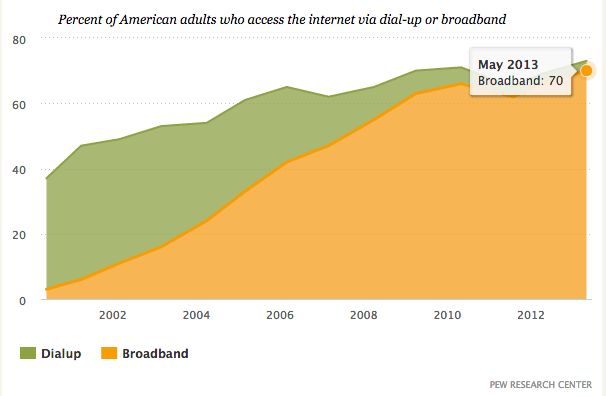
\includegraphics[width=0.6\textwidth]{figures/pew_internet_access}
\end{center}

\pause

\begin{itemize}
\item Each person in the poll be thought of as a \hl{trial}
\pause
\item A person is labeled a \hl{success} if s/he has high-speed broadband connection at home, \hl{failure} if not
\pause
\item Since 70\% have high-speed broadband connection at home, \hl{probability of success} is \hl{p = 0.70}
\end{itemize}

\end{frame}

% %%%%%%%%%%%%%%%%%%%%%%%%%%%%%%%%%%%

\begin{frame}
\frametitle{Considering many scenarios}

\disc{Suppose we randomly select three individuals from the US, what is the probability that exactly 1 has high-speed broadband connection at home?}

Let's call these people Anthony (A), Barry (B), Cam (C). Each one of the three
scenarios below will satisfy the condition of ``exactly 1 of them says Yes'': \\
\vspace{0.25cm}
\pause
\begin{changemargin}{+1.5cm}{+0cm}
{\footnotesize
\begin{enumerate}
\item[Scenario 1:] $\slot{0.70}{\text{(A) \red{yes}}} \times \slot{0.30}{\text{(B) no}} \times \slot{0.30}{\text{(C) no}} \approx 0.063$
\pause
\item[Scenario 2:]  $\slot{0.30}{\text{(A) no}} \times \slot{0.70}{\text{(B) \red{yes}}} \times \slot{0.30}{\text{(C) no}} \approx 0.063$
\pause
\item[Scenario 3:]  $\slot{0.30}{\text{(A) no}} \times \slot{0.30}{\text{(B) no}} \times \slot{0.70}{\text{(C) \red{yes}}} \approx 0.063$
\end{enumerate}
}
\end{changemargin}
\pause
The probability of exactly one 1 of 3 people saying Yes is the sum of all of these probabilities.
\[ 0.063 + 0.063 + 0.063 = 3 \times 0.063 = 0.189 \]

\end{frame}

%%%%%%%%%%%%%%%%%%%%%%%%%%%%%%%%%%%

\begin{frame}
\frametitle{Binomial distribution}

The question from the prior slide asked for the probability of given number of successes, \mathhl{k}, in a given number of trials, \mathhl{n}, ($k = 1$ success in $n = 3$ trials), and we calculated this probability as
\[ \#~of~scenarios \times P(single~scenario) \]

\pause

\begin{itemize}

\item $P(single~scenario) = p^k~(1-p)^{(n-k)}$ \\
{\tiny probability of success to the power of number of successes, probability of failure to the power of number of failures}

\pause

\item number of scenarios: ${n \choose k} = \frac{n!}{k! (n - k)!}$

\end{itemize}

\pause
$\:$ \\

The \hl{Binomial distribution} describes the probability of having exactly $k$
successes in $n$ independent trials with probability of success $p$.

\end{frame}

%%%%%%%%%%%%%%%%%%%%%%%%%%%%%%%%%%%

\begin{frame}[fragile]
\frametitle{Binomial distribution (cont.)}

\[P(k~successes~in~n~trials) = {n \choose k}~p^k~(1-p)^{(n-k)} \] 

\pause

\Note{You can also use R for the calculation of number of scenarios:}
{\footnotesize
\begin{Verbatim}[frame=single, formatcom=\color{blue}]
> choose(5,3)
\end{Verbatim}
}
{\footnotesize
\begin{Verbatim}[frame=single, formatcom=\color{gray}]
[1] 10
\end{Verbatim}
}
\pause
\Note{And to compute probabilities}
{\footnotesize
\begin{Verbatim}[frame=single, formatcom=\color{blue}]
> dbinom(1, size = 3, prob = 0.7)
\end{Verbatim}
}
{\footnotesize
\begin{Verbatim}[frame=single, formatcom=\color{gray}]
[1] 0.189
\end{Verbatim}
}

\end{frame}

%%%%%%%%%%%%%%%%%%%%%%%%%%%%%%%%%%%

\begin{frame}

\clicker{Which of the following is not a condition that needs to be met for the binomial distribution to be applicable?}

\begin{enumerate}[(a)]
\item the trials must be independent
\item the number of trials, $n$, must be fixed
\item each trial outcome must be classified as a \textit{success} or a \textit{failure}
\item \solnMult{the number of desired successes, $k$, must be greater than the number of trials}
\item the probability of success, $p$, must be the same for each trial
\end{enumerate}

\end{frame}

%%%%%%%%%%%%%%%%%%%%%%%%%%%%%%%%%%%

\begin{frame}
\frametitle{}

\clicker{According to the results of the Pew poll suggesting that 70\% of Americans have high-speed broadband connection at home, is the probability of exactly 2 out of 15 randomly sampled Americans having such connection at home pretty high or pretty low?}

\begin{enumerate}[(a)]
\item pretty high
\item \solnMult{pretty low}
\end{enumerate}

\end{frame}

%%%%%%%%%%%%%%%%%%%%%%%%%%%%%%%%%%%%

\begin{frame}

\clicker{According to the results of the Pew poll 70\% of Americans have high-speed broadband connection at home, what is the probability that exactly 2 out of 15 randomly sampled Americans have such connection at home?}

\begin{enumerate}[(a)]
\item $0.70^{2} \times 0.30^{13}$

\item ${2 \choose 15} \times 0.70^{2} \times 0.30^{13}$

\item \solnMult{${15 \choose 2} \times 0.70^{2} \times 0.30^{13}$} \soln{\red{\only<2>{$ = \frac{15!}{13! \times 2!} \times  0.70^{2} \times 0.30^{13} = 105 \times  0.70^{2} \times 0.30^{13} = 8.2e-06$}}}

\item ${15 \choose 2} \times 0.70^{13} \times 0.30^2$

\end{enumerate}

\end{frame}

%%%%%%%%%%%%%%%%%%%%%%%%%%%%%%%%%%%

\subsection{Expected value and standard deviation of the binomial can be calculated using its parameters n and p}
\label{mi5}

%%%%%%%%%%%%%%%%%%%%%%%%%%%%%%%%%%%%

\begin{frame}
\frametitle{Expected value and standard deviation of binomial}

\disc{According to the results of the Pew poll suggestion that 70\% of Americans have high-speed broadband connection at home, among a random sample of 100 Americans, how many would you expect to have such connection at home?}

\pause

\begin{itemize}

\item $100 \times 0.70 = 70$
\pause
\begin{itemize}
\item Or more formally, $\mu = np = 100 \times 0.7 = 7$
\end{itemize}

\pause

\item But this doesn't mean in every random sample of 100 Americans exactly 70 will have high-speed broadband connection at home. In some samples there will be fewer of those, and in others more. How much would we expect this value to vary?
\pause
\begin{itemize}
\item $\sigma = \sqrt{np(1-p)} = \sqrt{100 \times 0.70 \times 0.30} \approx  4.58$
\end{itemize}

\end{itemize}

\Note{Mean and standard deviation of a binomial might not always be whole numbers, and that is alright, these values represent what we would expect to see on average.}

\end{frame}


%%%%%%%%%%%%%%%%%%%%%%%%%%%%%%%%%%%

\subsection{Shape of the binomial distribution approaches normal when the S-F rule is met}
\label{mi6}

%%%%%%%%%%%%%%%%%%%%%%%%%%%%%%%%%%%%

\begin{frame}
\frametitle{Shape of the binomial distribution}

\vfill

\begin{center}
\webURL{https://gallery.shinyapps.io/dist_calc/}
\end{center}
\vfill

\pause

You can use the normal distribution to approximate binomial probabilities when
the sample size is large enough.

\hfill \\

\pause

\hl{S-F rule:} 
The sample size is considered large enough if the expected number of successes and failures are both at least 10
\[ np \ge 10 \qquad \text{ and } \qquad n(1-p) \ge 10 \]

\end{frame}

%%%%%%%%%%%%%%%%%%%%%%%%%%%%%%%%%%%

\begin{frame}[fragile]
\frametitle{}

\disc{What is the probability that among a random sample of 1,000 Americans at
least three-fourths have high-speed broadband connection at home?}

\vspace{-0.5cm}
\pause

\[ Binom(n = 1000, p = 0.7) \]
\vspace{-1cm}

\pause

{\small \[ P(K \ge 750) = P(K = 750) + P(K = 751) + P(K = 752) + \cdots + P(K = 1000) \]}

\pause

\begin{enumerate}

\item Using R:
{\footnotesize
\begin{Verbatim}[frame=single, formatcom=\color{blue}]
> sum(dbinom(750:1000, size = 1000, prob = 0.7))
\end{Verbatim}
}
{\footnotesize
\begin{Verbatim}[frame=single, formatcom=\color{gray}]
[1] 0.00026
\end{Verbatim}
}

\pause

\item Using the normal approximation to the binomial: Since we have at least expected successes
$(1000 \times 0.7 = 700)$ and 10 expected failures $(1000 \times 0.3 = 300)$,

\begin{align*}
Binom&(n = 1000, p = 0.7) \sim \\
&N(\mu = 1000 \times 0.7, \sigma = \sqrt{1000 \times 0.7 \times 0.3}) 
\end{align*}

\end{enumerate}

\end{frame}

%%%%%%%%%%%%%%%%%%%%%%%%%%%%%%%%%%%%

\section{Summary}

%%%%%%%%%%%%%%%%%%%%%%%%%%%%%%%%%%%%

\begin{frame}
\frametitle{Summary of main ideas}

\vfill

\begin{enumerate}

\item \nameref{mi1}

\item \nameref{mi2}

\item \nameref{mi3}

\item \nameref{mi4}

\item \nameref{mi5}

\item \nameref{mi6}

\end{enumerate}

\vfill

\end{frame}

%%%%%%%%%%%%%%%%%%%%%%%%%%%%%%%%%%%

\end{document}